\section{Value-based RL: Learning with approximation}
\label{sec:value_based_approximation}
\textit{This section reviews the lecture slides 5 and 6.}
\begin{itemize}
	\item When we talk about approximating the value function, we mean that instead of implementing $v$ as look-up table, we view it as parameterized function $\hat{v}(\bm{w},s)\approx v_{\pi}(s)$ with $\bm{w}\in\R^{d}$.
	\item Commonly, we try to allow generalization over nearby states while trying to keep it compact. Hence, the size of the weights,  $d$, is mostly much smaller than the actual state size. This implies that a change in $\bm{w}$ will affect many states, and hence, generalize.
	\item Learning value functions is similar to supervised learning as we try to push a prediction closer to a target (similar to regression). The value error can be summarized as:
	$$\overline{\text{VE}}(\bm{w}) = \sum_{s\in S}\mu(s)\left[v_{\pi}(s)-\hat{v}(s,\bm{w})\right]^2=\E_{s\sim\mu(s)}\left[\left(v_{\pi}(s)-\hat{v}(s,\bm{w})\right)^2\right]$$
	where $\mu(s)$ is a weighting factor for the states (which state is how important, distribution over those). This depends on the task we are aiming for.
	
	However, keep in mind that our overall goal is to find the optimal policy, and not the best value function. So, the VE error might not be optimal as we often converge to local optima. 
\end{itemize}
\subsection{Types of function approximations}
\begin{itemize}
	\item There are various function approximation techniques we can use. We will review here a few, practical/simple ones
	\item In general, we distinguish between linear and non-linear function approximation. We call an approximation linear if the value function is linear with respect to the weight, namely:
	$$\hat{v}(s,\bm{w})=\bm{w}^T\bm{x}(s)$$
	where $\bm{x}(s)$ can be any (non-)linear functions. It can be also seen as a linear combination of static feature extractions. Some examples for $\bm{x}$ are:
	\begin{itemize}
		\item \textit{Polynomials}, as if we take enough (infinite), we would be able to approximate any function. However, this is not feasible so we mostly have many features (especially in higher dimensions because we have $\left[1,s_1,s_2,s_1^2, s_2^2, s_1s_2, s_1^2s_2,...\right]$), and hence less generalization. Furthermore, the behavior at 0 is rather static
		\item \textit{Aggregations} where we group multiple states into one. This can be seen as returning a one-hot vector for $\bm{x}$ where the $1$ assigns a point to a certain state group. Figure~\ref{fig:rl_approximate_value_based_aggregation} visualizes some examples.
		\begin{figure}[ht!]
			\centering
			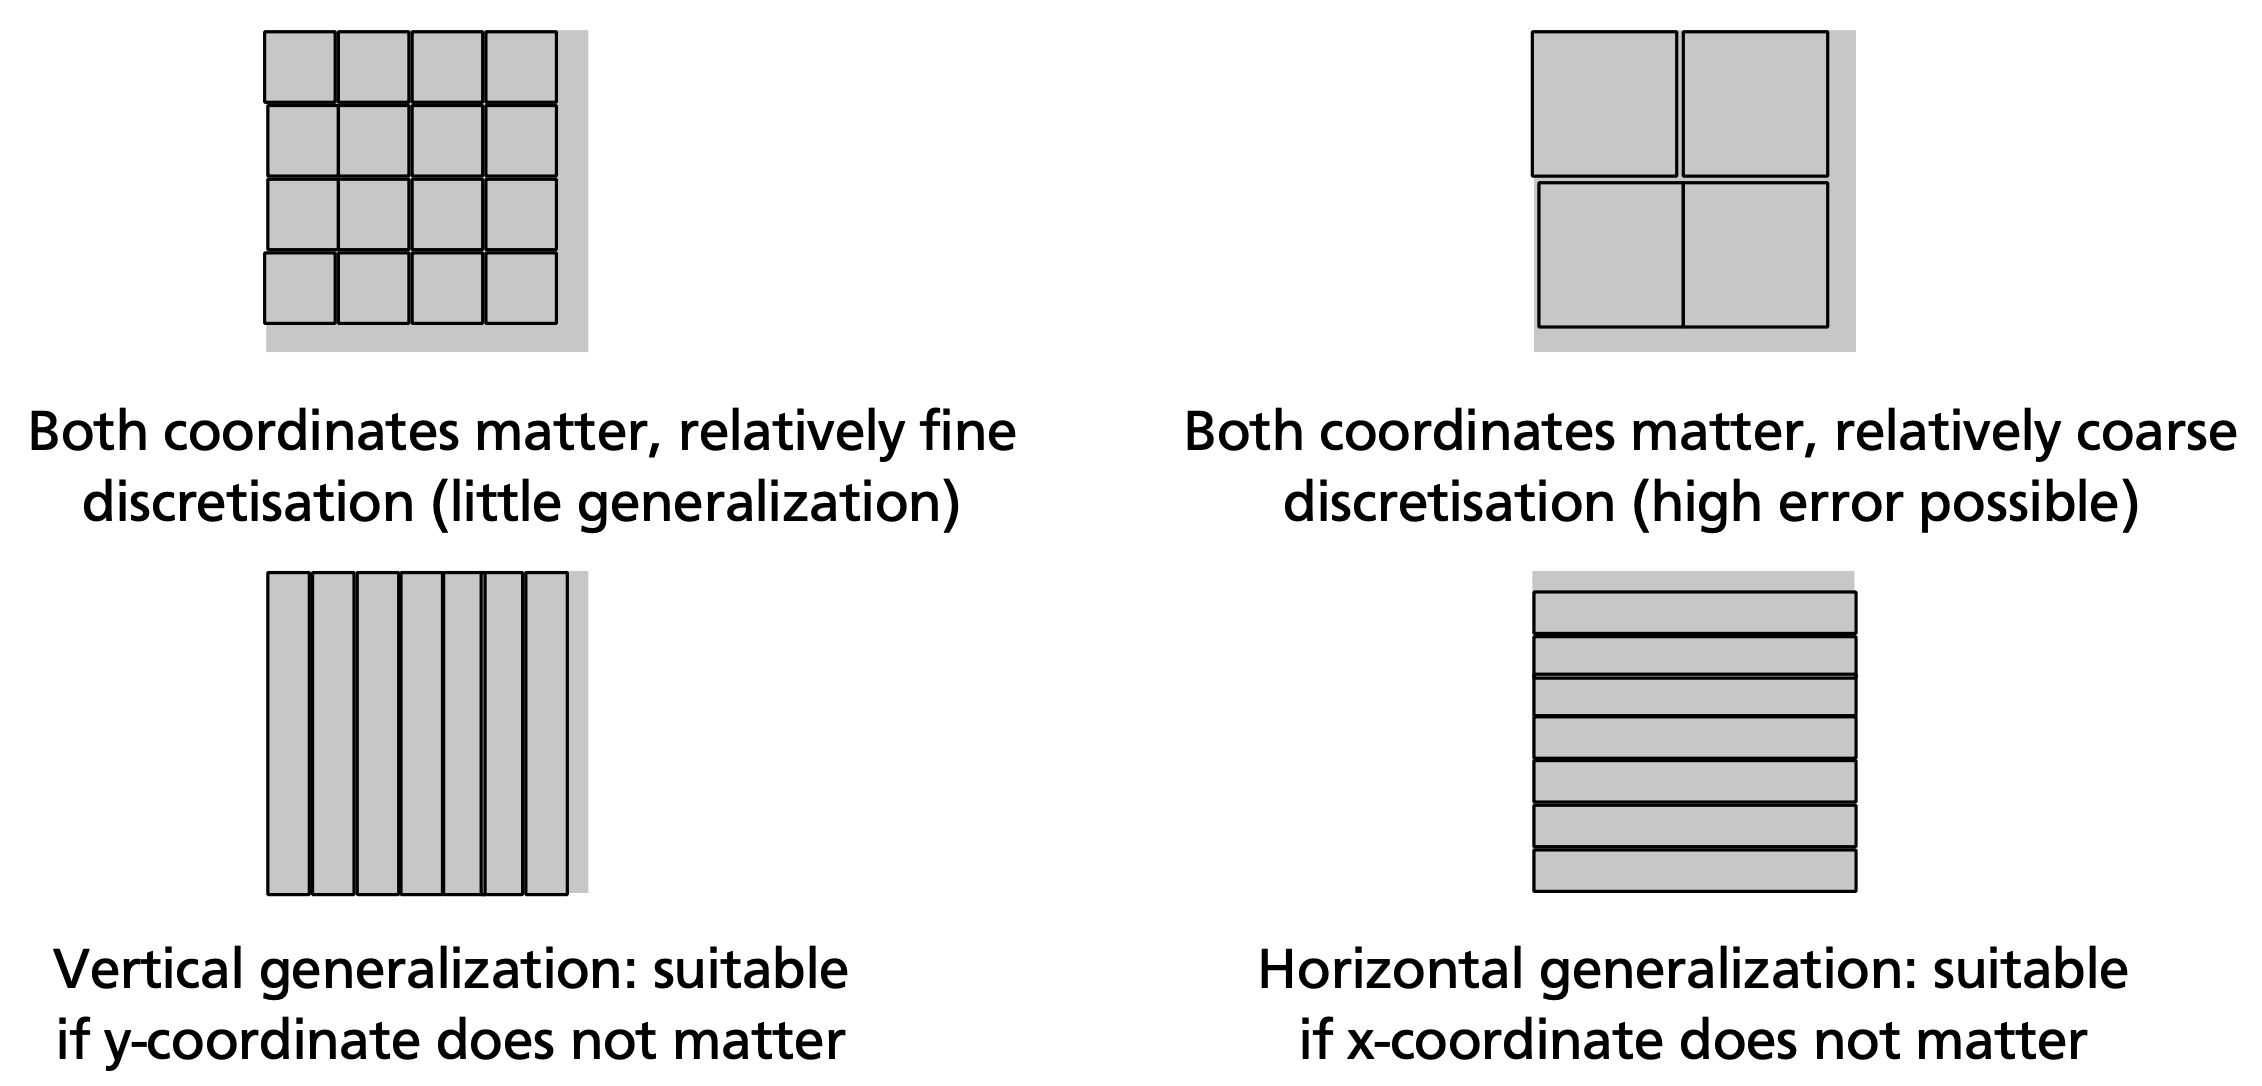
\includegraphics[width=0.5\textwidth]{figures/rl_approximate_value_based_aggregation.png}
			\caption{Simple types of aggregations on a 2D state space. Note that we can combine aggregations, meaning that we use both a vertical and a horizontal aggregation.}
			\label{fig:rl_approximate_value_based_aggregation}
		\end{figure}
		\item \textit{Radial basis functions} that takes the distance to a mean in the state space, e.g. $||\mu_i-s||$, as input features. We can model this by having multiple Gaussian, and weight their influence by $p(s)$. It enables us to have smoother transitions between close-by states, but might be problematic for far-away states. This is why it is often problematic in high-dimensional state spaces.
		\item \textit{Fourier basis} where we take different frequencies to model $s$. This can provide a quite flexible feature set.
	\end{itemize}
	Note that tabular RL can also be expressed by linear function approximation where we simply use $\bm{x}(s)=\left[\delta(s=s_1), \delta(s=s_2),...\right]$, and $\bm{w}$ therefore contains one parameter per state.
	
	Linear function approximation is especially used when prior knowledge can be introduced in the system. Carefully selecting the features simplifies the learning objective of the model, and hence, let it converge faster.
	
	\item In non-linear function approximation, we use $\bm{w}$ in a non-linear fashion in $\hat{v}$, such as in neural networks.
	
\end{itemize}
\subsection{Prediction objective for on-policy prediction}
\begin{itemize}
	\item In the case that we perform a on-policy prediction (i.e. policy evaluation for a fixed policy), the state importance is based on the visit frequency of $\pi$. To arrive at $\mu$, we also have to distinguish between the tasks:
	\begin{itemize}
		\item If we have a continuing task (never ending), we get a stationary distribution at the point:
		$$\mu_{\pi}(s)=\sum_{s'}\sum_{a}p(s|s',a)\pi(a|s')\mu_{\pi}(s')$$
		with the condition that we can reach every state from the start.
		\item For episodic tasks, we need to consider the start frequency $h(s)$ as well. To guarantee that $\mu(s)$ is a distribution, we can use a softmax:
		$$\mu_{\pi}(s)=\frac{\eta(s)}{\sum_{s'}\eta(s')}, \hspace{4mm}\eta(s)=h(s)+\sum_{s'}\sum_a p(s|s',a)\pi(a|s')\eta(s')$$
		where the second part is pretty much the same as before.
	\end{itemize} 
	\item In order to calculate the gradients $\nabla_{\bm{w}}\overline{\text{VE}}(\bm{w})$, we would need to know $\mu(s)$ which is not possible due to missing information of the environment dynamics ($p(s'|s,a)$). However, we can approximate it by Monte-Carlo samples such that:
	$$\nabla_{\bm{w}}\overline{\text{VE}}(\bm{w})\approx \nabla_{\bm{w}}\left[G_t - \hat{v}(S_t,\bm{w})\right]^2 = -2\cdot \left[G_t - \hat{v}(S_t,\bm{w})\right] \nabla_{\bm{w}}\hat{v}(S_t,\bm{w})$$
	Which leads us to the \textbf{Gradient Monte Carlo} algorithm:
	$$\bm{w}_{t+1}=\bm{w}_{t}+\alpha \left[G_t - \hat{v}(S_t,\bm{w})\right] \nabla_{\bm{w}}\hat{v}(S_t,\bm{w})$$
	\item Alternatively, we could also think about using the bootstrapping estimate as target, which gives us the following update rule:
	$$\bm{w}_{t+1}=\bm{w}_t + \alpha\underbrace{\left[R_{t+1} + \gamma\hat{v}(S_{t+1},\bm{w}_t) - \hat{v}(S_t,\bm{w}_t)\right]}_{\text{TD error }\delta}\nabla_{\bm{w}}\hat{v}(S_t,\bm{w}_t)$$  
	This method is called \textbf{Semi-gradient TD(0)}, and indicates by its name that it is not a true gradient. The reason for that is that we actually ignore the dependency of the target on $\bm{w}$. We assume it to be fixed.  Nevertheless, experiments with the true gradient have shown that the semi-gradient works much better in practice. We will discuss it later in more detail.
	
	Note that as in the value-based, we can extend this approach to $n$-step if wanted.
	\item When comparing Gradient MC and semi-gradient TD(0), we get the same arguments as for the tabular case in Section~\ref{sec:value_based_tabular_difference_TD_MC} $\Rightarrow$ TD has lower variance and learns usually faster, but can have a bias (see below)
	\item A thing to keep in mind when using semi-gradient TD(0) is that it tries to minimize distance between close-by states, especially if we take approximation like aggregating multiple state into the same. This is because a small step can lead to a huge TD error which we try to minimize. 
	\begin{figure}[ht!]
		\centering
		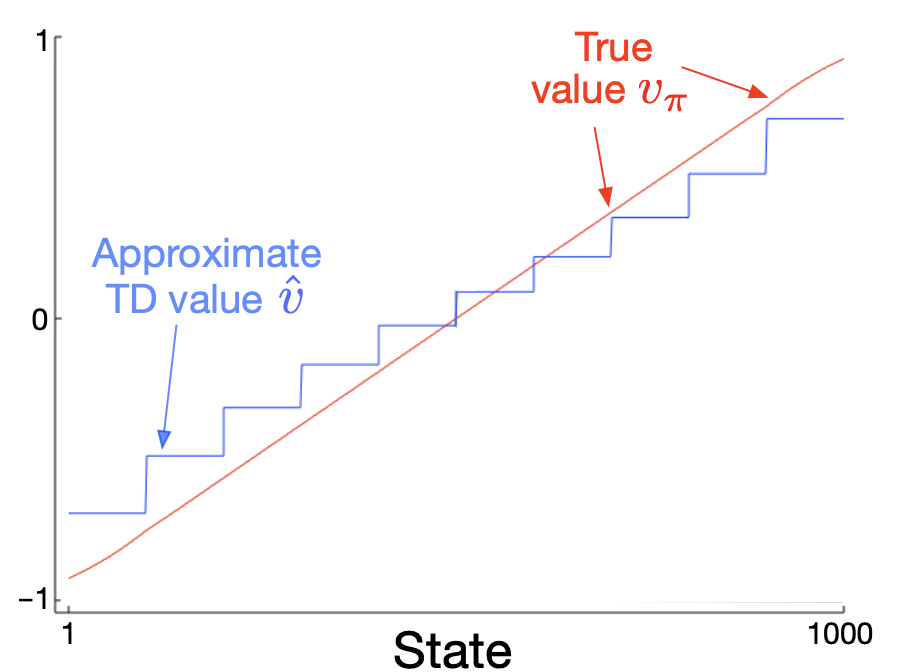
\includegraphics[width=0.4\textwidth]{figures/rl_approximate_value_based_semi_gradient_td.png}
		\caption{Problems of semi-gradient TD(0) updates on the random walk example. It prefers a value function with low changes between states, so that it gets a biased prediction.}
		\label{fig:rl_approximate_value_based_semi_gradient_td}
	\end{figure}
\end{itemize}
\subsubsection{Discussion on convergence for different objectives}
\begin{itemize}
	\item The advantages of linear function approximations are that the gradients are easy to calculate ($\nabla_{\bm{w}}\hat{v}(s,\bm{w})=\bm{x}(s)$). Furthermore, it can be proven that all local optima are global optima, so that gradient MC converges to the minimum of $\overline{\text{VE}}$. This is not necessarily the case for semi-gradient TD but we can define a upper bound $\overline{\text{VE}}(\bm{w}_{td})\leq \frac{1}{1-\gamma}\min_{\bm{w}}\overline{\text{VE}}(\bm{w})$ and guarantee that it converges. 
	
	In the non-linear case, we cannot guarantee convergence for semi-gradient TD (but for Gradient Monte Carlo), and we might end up in local optima. Nevertheless, linear features are much more restricted than non-linear as neural networks. Hence, non-linear methods can lead to better results, even if we might get stuck in local optima.
	
	\item When learning via Gradient Monte Carlo or Semi-gradient TD, we have to select a step size $\alpha$. This can be a bit more tricky here because we combine the values of many states into a single function. In case of linear function approximation, we can actually give a rule of thumb because the features are static, namely:
	$$\alpha = (\tau\E[\bm{x}^T\bm{x}])^{-1}$$
	where $\tau$ is the number of experiences we expect to have for the same (or similar) feature vector to average over (as say the learning rate you would choose for the tabular setting would be $\frac{1}{\tau}$)
	\item Alternatively we could try to find the fix point of semi-gradient TD(0). We can write the TD update rule for linear function approximation as:
	\begin{equation*}
		\begin{split}
			\bm{w}_{t+1} & = \bm{w}_t + \alpha \left(R_{t+1}+\gamma \bm{w}_t^T \bm{x}_{t+1} - \bm{w}_t^T\bm{x}_t\right)\bm{x}_t\\
			& = \bm{w}_t + \alpha \left(R_{t+1}\bm{x}_t - \bm{x}_t (\bm{x}_t - \gamma \bm{x}_{t+1})^T \bm{w}_t\right)\\
			\implies \E[\bm{w}_{t+1}|\bm{w}_t] & = \bm{w}_t + \alpha \left(\underbrace{\E[R_{t+1}\bm{x}_t]}_{\bm{b}} - \underbrace{\E[\bm{x}_t (\bm{x}_t - \gamma \bm{x}_{t+1})^T]}_{\bm{A}} \bm{w}_t\right)\\
		\end{split}
	\end{equation*}
	The fix point is given when we do not change our weights anymore, meaning $\bm{w}_{t+1}=\bm{w}_t$. This is the case if:
	$$\bm{w}_{td}=\bm{A}^{-1}\bm{b}$$
	We can approximate $\bm{A}$ and $\bm{b}$ by MC sampling:
	\begin{equation*}
		\begin{split}
			\hat{\bm{A}}_t & = \sum_{k=0}^{t-1}\bm{x}_k\left(\bm{x}_k - \gamma\bm{x}_{k+1}\right)^T + \epsilon\bm{I}\\
			\hat{\bm{b}}_t & = \sum_{k=0}^{t-1}R_{k+1}\bm{x}_k
		\end{split}
	\end{equation*}
	where $\epsilon$ is a small constant ensuring that $\bm{\hat{A}}$ is always invertible. This solution is called \textbf{least-squares temporal-difference (LSTD)}, and is usually more sample efficient because we do not have to perform iterative updates, and has the benefit of not requiring a step size. However, it is more computationally expensive (quadratic plus the invert of $\bm{A}$), and we cannot adapt to a change in the environment over time (once performed, we fix our weights)
\end{itemize}
\subsection{Control with approximation}
\begin{itemize}
	\item For learning a policy $\pi$, we again change our objective to learning the $q$-values, which we now approximate with $\hat{q}(s,a,\bm{w})$. We will focus on episodic cases, but note that everything could be generalized to the continuous case as well.
	\item In the \textbf{on-policy} case, we can use methods like (episodic) semi-gradient SARSA, so that our update step is:
	$$\bm{w}_{t+1}=\bm{w}+\alpha\left[U_t - \hat{q}(S_t,A_t,\bm{w})\right]\nabla_{\bm{w}}\hat{q}(S_t,A_t,\bm{w})$$
	where $U_t$ is our target, which is for one-step SARSA $U_t = R_t + \gamma \hat{q}(S_{t+1},A_{t+1},\bm{w})$.
	As usual, we iterate over this update rule while setting our policy to $\epsilon$-greedy on $\hat{q}$.
	\item In the \textbf{off-policy} case, we experience more problems. As we have a behavior policy $b$ and target policy $\pi$, we often need to use importance weight to correct the target of the update:
	$$\bm{w}_{t+1}=\bm{w}_{t}+\rho \alpha\left[U_t - \hat{q}(S_t,A_t,\bm{w})\right]\nabla_{\bm{w}}\hat{q}(S_t,A_t,\bm{w})$$
	Although it increases variance, it is sometimes necessary to guarantee unbiased, correct estimates. However, note that in cases like Q-learning, where $U_t$ is independent of $b$, we might not have to consider the importance weights as $\rho=1$.
	
	The second issue is that we need to take the changed state distribution, $\mu_b$, into account. Consider for example the very simple MDP in Figure~\ref{fig:rl_approximation_value_based_offpolicy_divergence} for which we just want to estimate $v$ (policy evaluation). We assume the reward for any action to be $0$, and start with an initial value of $w=10$.
		
	\begin{figure}[ht!]
		\centering
		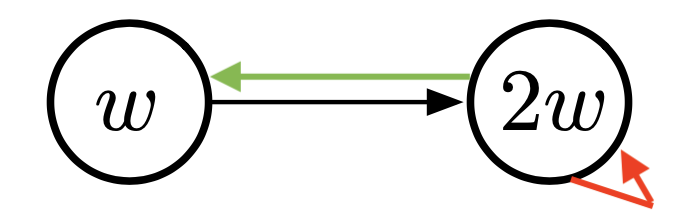
\includegraphics[width=0.2\textwidth]{figures/rl_approximation_value_based_offpolicy_divergence.png}
		\caption{Simple MDP where off-policy updates can diverge. Green indicate behavior policy, red the target. Every transition has a reward of $0$, meaning that the optimal $v$ are 0 at both states.}
		\label{fig:rl_approximation_value_based_offpolicy_divergence}
	\end{figure}
	
	First, consider the on-policy case where $\pi=b$ (green action from second state). Then, we would alternate between the two update equations:
	\begin{equation*}
		\begin{split}
		\text{Left to right: }\hspace{2mm}w_{t+1} & = w_t + \alpha (\gamma \cdot 2w_t-w_t)\nabla_w w_t = (1+\alpha(2\gamma-1)) w_t\\
		\text{Right to left: }\hspace{2mm}w_{t+1} & = w_t + \alpha (\gamma w_t-2w_t)\nabla_w 2w_t = (1+2\alpha(1-2\gamma)) w_t\\
		\end{split}
	\end{equation*}
	Overall, we would converge to $w=0$ as the right to left update is twice as high as the other.
	
	Now, assume the behavior policy stays the same, but our target policy stays at the second state. Then, the importance weight for left to right is 1 (as both policies do that with probability 1), but from right to left is zero because we would not take this action with our target policy. So we end up with the update:
	\begin{equation*}
		\begin{split}
			\text{Left to right: }\hspace{2mm}w_{t+1} & = w_t + \alpha (\gamma \cdot 2w_t-w_t)\nabla_w w_t = (1+\alpha(2\gamma-1)) w_t\\
		\end{split}
	\end{equation*}
	which makes $w_t$ head to infinity if $\gamma>0.5$. This shows that off-policy prediction can diverge!
	
	\item This divergence can occur when the following three methods are used together (\textit{Deadly Triad}):
	\begin{itemize}
		\item Function approximation
		\item Semi-gradient bootstrapping
		\item Off-policy training
	\end{itemize}
	\item To overcome this issue, we need to consider alternatives to semi-gradients.
	
\end{itemize}
\subsubsection{Alternatives to semi-gradients}
\begin{itemize}
	\item There are couple of objectives that we can use instead of semi-gradient. We visualize all of them in Figure~\ref{fig:rl_approximation_value_based_different_errors}, and discuss them here in detail
	\begin{figure}[ht!]
		\centering
		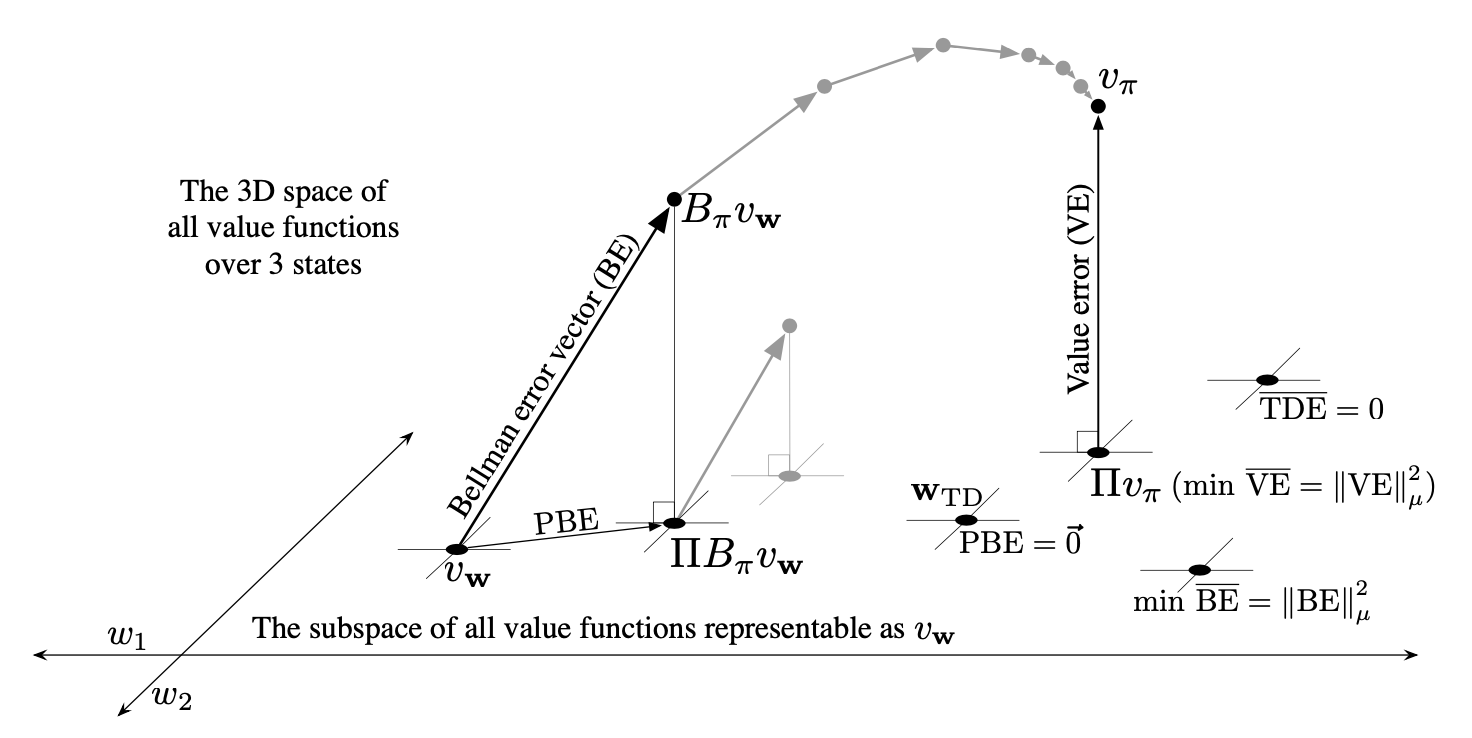
\includegraphics[width=0.6\textwidth]{figures/rl_approximation_value_based_different_errors.png}
		\caption{Geometry of linear value-function approximation. We show an approximation of a 3D state space by a two dimension weight vector.}
		\label{fig:rl_approximation_value_based_different_errors}
	\end{figure}
	
	\item Before we start our discussion, we need to introduce some notation:
	\begin{itemize}
		\item First, we need to consider how we measure distance between two value functions. The standard euclidean norm is not sufficient, as we give importance to different states. This is why we take $\mu$ into account:
		$$||v_1-v_2||_{\mu}^2 = \sum_{s\in\mathcal{S}} \mu(s)\left[v_1(s)-v_2(s)\right]^2$$
		\item Given the norm, we also want to define a \textit{projection operator} which assign to an arbitrary $v$ (over whole state space) the closest value function based on the norm that can be represented:
		$$\Pi v = v_{\bm{w}}\hspace{3mm}\text{where}\hspace{3mm}\bm{w}=\arg\min_{\tilde{\bm{w}}}||v-v_{\tilde{\bm{w}}}||_{\mu}^2 $$
		\item The last notation we want to introduce is the Bellman operator, which maps a value function $v$ to its bootstrapping estimates:
		$$(B_{\pi}v_{\bm{w}})(s) = \sum_a \pi(a|s)\sum_{s',r}p(s',r|s,a)[r+\gamma v_{\bm{w}}(s')] = v_{\bm{w}}(s) + \overline{\delta}_{\bm{w}}(s)$$
		with $\overline{\delta}_{\bm{w}}(s)$ being the expected TD error for state $s$.
	\end{itemize}
	\item The value error $\overline{\text{VE}}$ is minimized if the norm is the lowest to $v_{\pi}$: $$\min_{\bm{w}} \overline{\text{VE}}(\bm{w}) = \min_{\bm{w}} ||v_{\bm{w}}-v_{\pi}||_{\mu}^2 $$
	The projected point, which we can actually reach, is $\Pi v_{\pi}$ which is the best point we can represent in our $\bm{w}$-space. Gradient Monte Carlo methods converge to this point, but mostly quite slowly
	\item Without the approximation, we could simply apply the Bellman operator  over and over again, and reach $v_{\pi}$ (as in tabular TD(0) learning) which is the gray line above. However, we cannot represent the change so that we have to project $v$ after each step: $\Pi B_{\pi}v_{\bm{w}}$. The step we take in between is the projected Bellman error $PBE=\Pi\delta_{\bm{w}}$ 
	
	Semi-gradient TD is converging to the point where $PBE=0$ as we reach a fix-point there. However, this does not have to be where the minimum Bellman error is reached because imagine $\delta_{\bm{w}}$ being orthogonal to $\bm{w}$-subspace. Then, the projected bellman error is 0, but without projection, we would continue changing $\bm{w}$, until we reach $\min \overline{\text{BE}}$.
	
	At the same time, even if we would reach $\min \overline{\text{BE}}$, it would be most likely not be a optimum (i.e. gradients greater than zero) because the gradients can point to outside the representable $\bm{w}$-space (does not need to be orthogonal as before), and hence the projected Bellman error can be unequals zero.
	
	\item The last objective we consider here is the true-gradient TD error, meaning: $$\overline{\text{TDE}}(\bm{w})=\sum_{s\in\mathcal{S}}\mu(s)\E\left[\delta_t^2 |S_t=s,A_t\sim \pi\right] = \E_{b}[\rho_t \delta_t^2] \hspace{4mm}\text{(if we assume $\mu$ is under $b$)}$$
	Following SGD updates, we get:
	$$\bm{w}_{t+1}=\bm{w}_t + \alpha \rho_t \delta_t (\nabla \hat{v}(S_t,\bm{w}_t) - \gamma \nabla \hat{v}(S_{t+1},\bm{w}_t))$$
	
	\item Now, let's consider which of these objectives we can take as alternative to semi-gradient updates. 
	
	A major drawback of TDE is that we also take the gradients regarding the next steps, which can push the value function in a wrong direction (tries to minimize distance between the steps, similar to Figure~\ref{fig:rl_approximate_value_based_semi_gradient_td}). Consider the MDP in Figure~\ref{fig:rl_approximation_value_based_TDE}, with on-policy evaluation of a uniform policy, and $\gamma=1$.
	
	\begin{figure}[ht!]
		\centering
		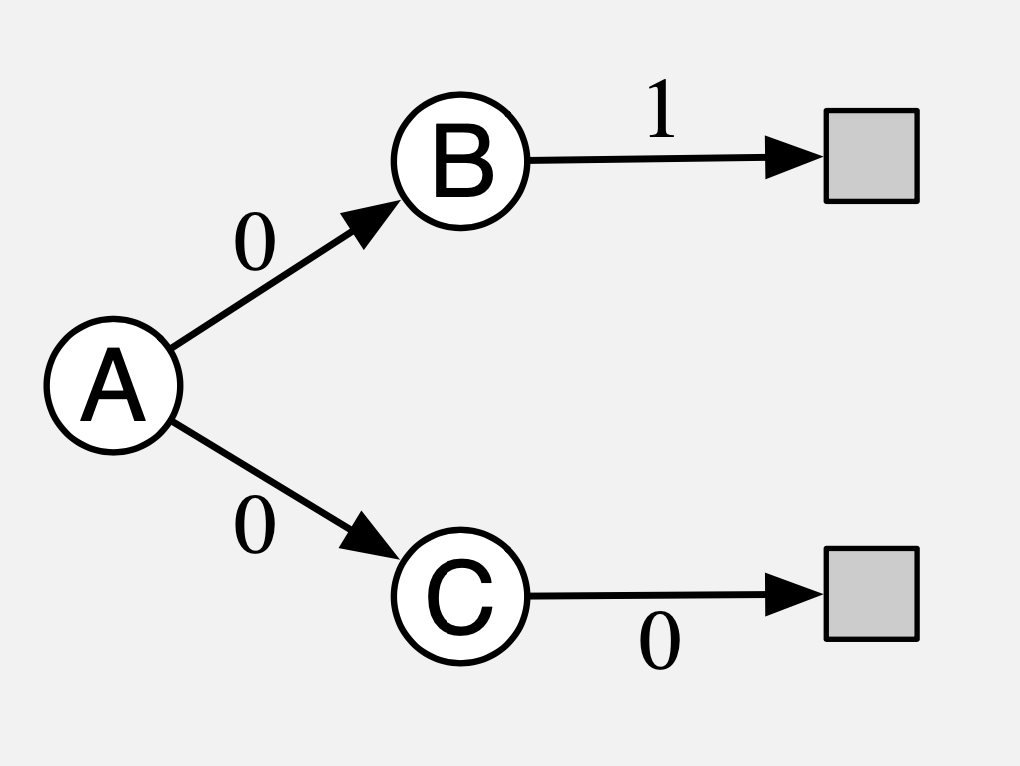
\includegraphics[width=0.2\textwidth]{figures/rl_approximation_value_based_TDE.png}
		\caption{Simple example where TDE gives an undesirable result.}
		\label{fig:rl_approximation_value_based_TDE}
	\end{figure}

	The optimal/correct value function is obviously $v(A)=1/2, v(B)=1, v(C)=0$. The TD error is given by:
	$$\delta_t=\frac{1}{2}\left(\left[v(B)-v(A)\right]^2 + \left[1-v(B)\right]^2\right)+\frac{1}{2}\left(\left[v(C)-v(A)\right]^2 + \left[0-v(C)\right]^2\right)$$
	for which the optimal is actually $v(A)=1/2, v(B)=3/4, v(C)=1/4$ because we also minimize the distance between $v(A)$ and $v(B)$, and similarly between $v(A)$ and $v(C)$.
	
	\item For calculating the Bellman error ($\min \text{BE}$), we need to calculate:
	$$\overline{\text{BE}}=||\overline{\delta}_{\bm{w}}||_{\mu}^2\hspace{2mm}\text{where}\hspace{2mm}\overline{\delta}_{\bm{w}}=\E_{\pi}\left[\delta_{\bm{w}}|S_t=s,A_t\sim\pi\right]$$
	As we have the square in the error, to guarantee an unbiased estimate, we need to sample at least two times independently (otherwise we estimate $\E[\delta^2]$ instead of $\E[\delta]^2$). This is mostly not possible in interactions to obtain, or makes the algorithm rather slow.
	
	\item The last remaining objective is the mean squared projected Bellman error $\overline{\text{PBE}}$. We can derive at the following gradient for PBE:
	$$\nabla_{\bm{w}} \overline{\text{PBE}}(\bm{w}) = 2\E[\rho_t (\gamma \bm{x}_{t+1}-\bm{x}_t)\bm{x}_t^T]\E[\bm{x}_t\bm{x}_t^T]^{-1}\E[\rho_t\delta_t\bm{x}_t]$$
	Using the same samples for all the expectations gives the same bias as the one for the Bellman error. What we can do, however, is learning some factors from all the data, namely the last two, and denote it as $\bm{v}_t=\E[\bm{x}_t\bm{x}_t^T]^{-1}\E[\rho_t\delta_t\bm{x}_t]$. Then, we can perform SGD as:
	\begin{equation*}
		\begin{split}
			\bm{v}_{t+1} & = \bm{v}_t + \beta \rho_t (\delta_t - \bm{v}_t^T \bm{x}_t)\bm{x}_t\\
			\bm{w}_{t+1} & = \bm{w}_t + \alpha \left[\rho_t (\gamma \bm{x}_{t+1}-\bm{x}_t)\bm{x}_t^T\right]\bm{v}_t
		\end{split}
	\end{equation*}
	This algorithm is called GTD2 (gradient TD) which converges to the minimum PBE for linear features. The drawbacks are that we need an additional learning rate $\beta$ (mostly greater than $\alpha$), and need to store two parameter updates.
	
	Nevertheless, as we have a guarantee of convergence for all settings, it makes GTD2 the preferred technique compared to Semi-gradient TD, except when we just want a simple method.
	\item Overall, we have the following convergence properties:
	\begin{figure}[ht!]
		\centering
		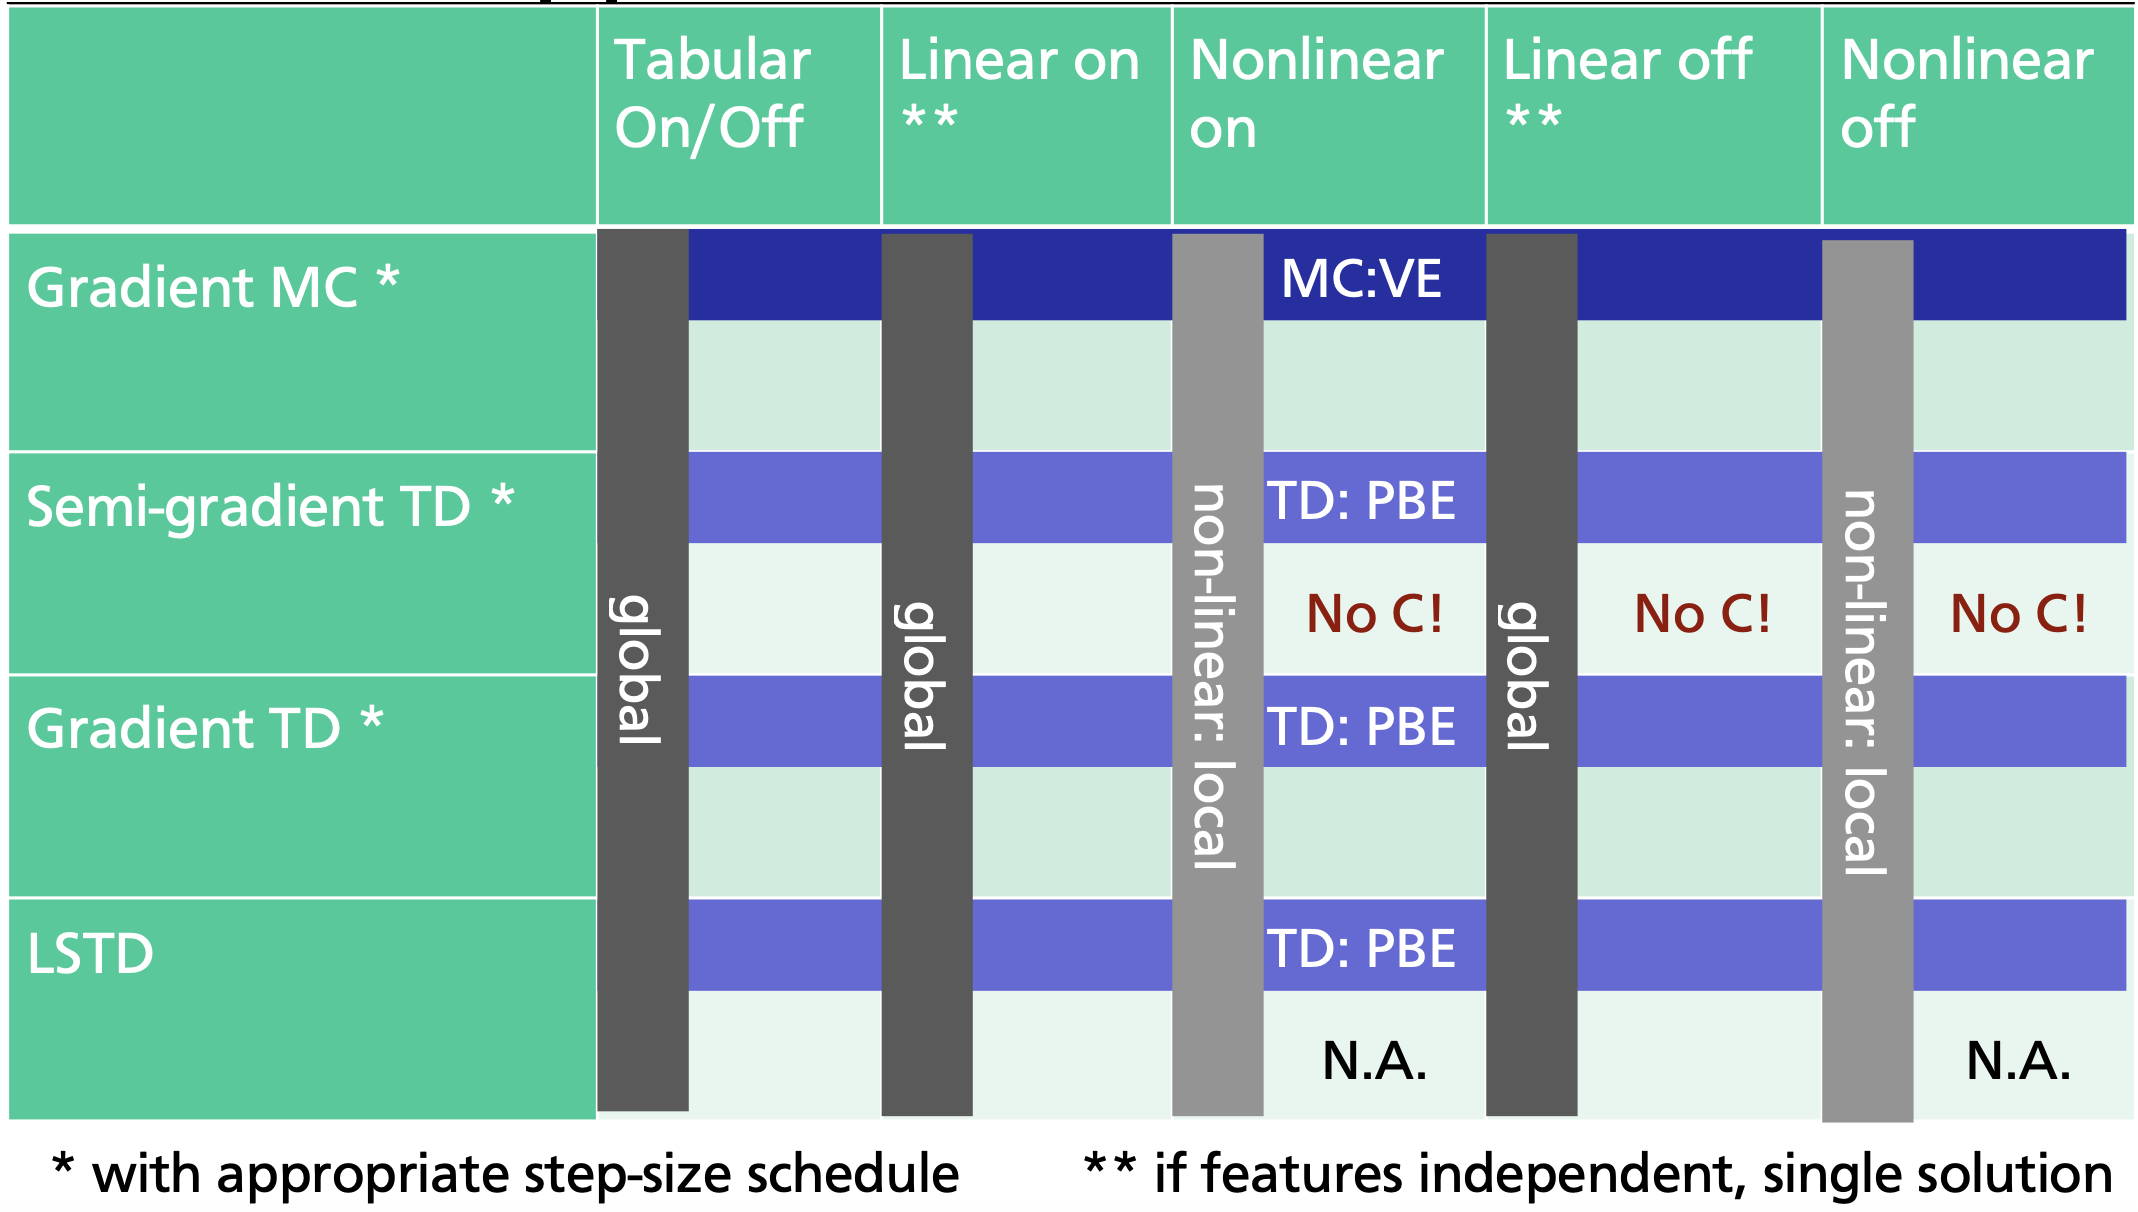
\includegraphics[width=0.6\textwidth]{figures/rl_approximate_value_based_convergence_overview.png}
		\caption{Overview of convergence properties of different optimization methods. The columns show the setting (on=on-policy, off=off-policy). "No C." for semi-gradient TD means that we cannot guarantee its convergence. "N.A" stands for "not applicable", as LSTD is based on the assumption of linear features.}
	\end{figure}	
\end{itemize}
\subsubsection{Deep Q network}
\begin{itemize}
	\item Another way of stabilizing off-policy control is by using many additional tricks, to make it more similar to supervised learning. One popular example of this is the DQN
	\item Given a state as input, we try to learn a $q$-value for each output, so that we can perform a simple maximization step over the outputs to get the optimal policy
	\item We use image as input. However, to detect movement, a couple of frames are stacked on top of each other
	\item To guarantee i.i.d. samples within a batch, and use data more efficiently (look at an experience more than once), we use \textbf{experience replay}:
	\begin{itemize}
		\item All the experiences we had from interacting with the environment are stored in a buffer (if limited size, use FIFO queue)
		\item At every time step, randomly select $N$ experiences which form a batch for training
	\end{itemize}
	Note that this is only possible because of off-policy training, as the collected experiences come from a different policy, namely an older one.
	\item Another trick to stabilize learning is \textbf{fixing the target}. As we use semi-gradient version of $q$-learning, which is:
	$$\bm{w}_{t+1}\leftarrow \bm{w}_t + \alpha \left[R_{t+1}+\gamma\max_a \hat{q}(S_{t+1}, a, \bm{w}_t) - \hat{q}(S_t, A_t, \bm{w}_t)\right]\nabla \hat{q}(S_t, A_t, \bm{w}_t)$$
	To fix the target, we copy the weights $\tilde{\bm{w}}$, and use this to calculate the target $\gamma\max_a \hat{q}(S_{t+1}, a, \bm{w}_t)$.
	
	Furthermore, it has been shown to work well to clip the TD error between a range of $[-1,1]$ to prevent any divergence issues. 
	\item If needed/wanted, we can overcome the maximization by using a double Q-learning approach
\end{itemize}





